\documentclass[a4paper,10pt]{article}
\usepackage[utf8]{inputenc}
\usepackage{graphicx}
\usepackage{booktabs}
\usepackage{rotating}
\usepackage{subfigure}
\bibliographystyle{plos2009}%
%opening
\title{Text S2 -- Assessing the impact of taxon sampling on phylogeographic reconstruction} % aargh, lousy name
\author{
Luiz Max de Carvalho \\
\and Nuno Faria \\
\and Guy Baele\\
\and Andres Perez \\
\and Philippe Lemey \\
\and Waldemir Silveira 
}
\date{}
\begin{document}

\maketitle

\section{Background}
The data sets used in this study presented high preferentiality of sampling, with some countries being overrepresented.
% A possibility, unexplored in this paper, is to sample each location with probability proportional to its disease prevalence
% In theory, a Bayesian approach should offer a certain degree of protection against model mispecification and sampling bias by bla bla...
\section{Comparing rate matrices}
Sometimes \\
L1 and L2 norms
We thank Professor Marc A. Suchard (UCLA) for advice on this topic.\\
\section{Quantifying spatial signal extraction}
KL root for each subsample
\section{Bayesian Stochastic Search Variable Selection}
% TODO: put in the BSSVS plots !!!
\section{Parameter estimation without the overrepresented locations}
Additionally, we assessed the robustness of our temporal reconstruction by using only sequences from 2000 to present. For this analysis, we used the Gaussian Markov Random Field (GMRF) smoothing prior on coalescent times, also known as 'skyride' model. These results are presented in Figure~\ref{fig:only2000sky}.
% TODO: more discussion on this 

 \begin{figure}[h]
\begin{center}
\subfigure[A]{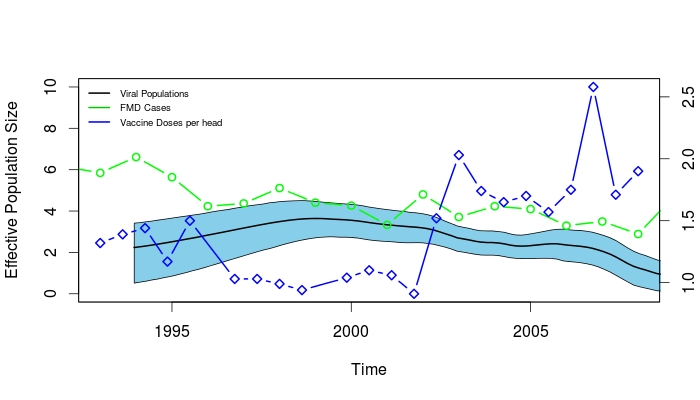
\includegraphics[width=\textwidth]{FIGURES/SFig_A2000sky.jpeg}}
\subfigure[O]{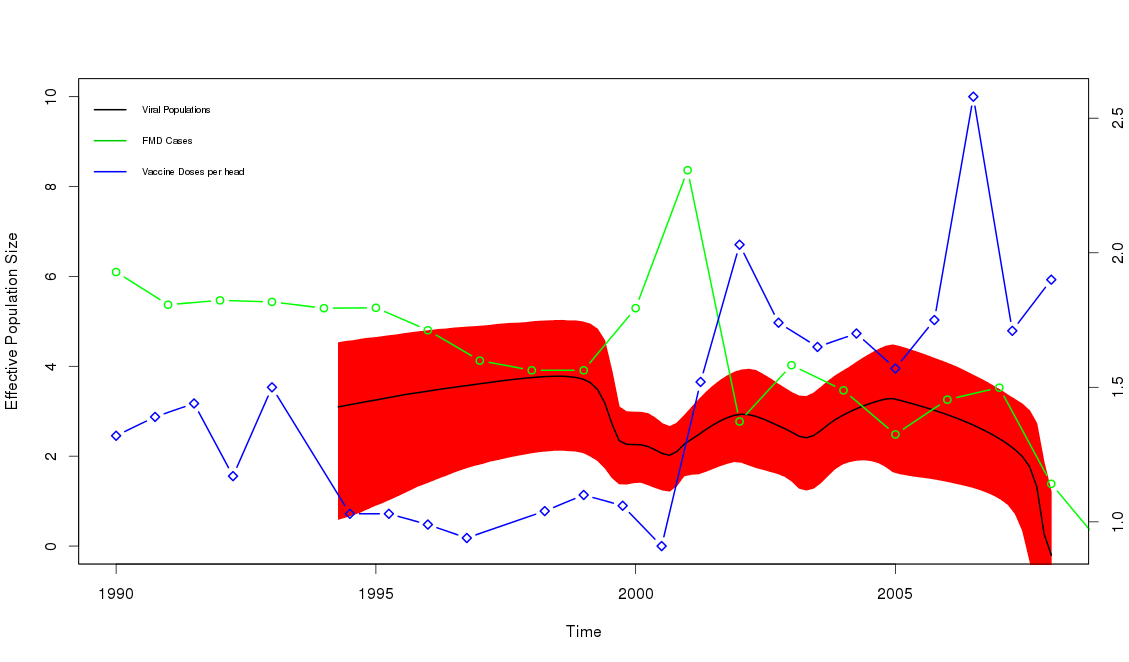
\includegraphics[width=\textwidth]{FIGURES/SFig_O2000sky.jpeg}}\\
\end{center}
\caption{}
\label{fig:only2000sky}
\end{figure}

\section{Parameter estimation with downsampling}
% For our experiments, we obtained five downsampled data sets for each serotype
\section{``Representation-informed'' priors}
\section{Simulating from the null}
\section{Results and Discussion}
\newpage
\section*{Table Legends}
\textbf{Table~\ref{tab:SB_A}. Parameter estimation using the complete and without Argentina data sets for serotype A} To assess the impact of the overrepresentation of Argentina in our sample we removed all sequence from this location and reestimated parameters. 1- All 131 sequences were used. 2- Time to most recent common ancestor. 3- Codon positions $1$, $2$ and $3$.

\textbf{Table~\ref{tab:SB_O}. Parameter estimation using the complete and without Ecuador data sets for serotype O} To assess the impact of the overrepresentation of Ecuador (90 sequences) our sample we removed all sequence from this location and reestimated parameters. 1- All 167 sequences were used. 2- Time to most recent common ancestor. 3- Codon positions $1$, $2$ and $3$.

\textbf{Table~\ref{tab:ED_A}. 'Equal downsampling' experiment for serotype A} Five random downsampled subsamples were obtained and used for parameter inference. 1-- $\times 10^{-3}$. 2 -- $\times 10^{-2}$. 3-- Probabily at root node. 

\textbf{Table~\ref{tab:ED_O}. 'Equal downsampling' experiment for serotype O} Five random downsampled subsamples were obtained and used for parameter inference. 1-- $\times 10^{-2}$. 2--  Probabily at root node.

\newpage
\section*{Figure Legends}

\textbf{Figure~\ref{fig:only2000sky}. Skyride coalescent reconstructions using sequences from 2000 to present only for both serotypes. As in the main text, disease cases and vaccination in doses per head are overlaid to the demographic reconstructions.} 

\newpage
\bibliography{Text_S2}
\newpage 

\begin{center}
\begin{table}[h]
\caption{}
\begin{tabular}{ccc}
\toprule
Parameter	&Complete$^{1}$	&Without Argentina\\
\midrule
TMRCA$^{2}$	&76.40 (69.48-83.65)	&82.31 (72.40-92.81)\\
CP1$	^{3}$	&0.65 (0.54-0.76)	&0.62 (0.51-0.75)\\
CP2	&0.46 (0.37-0.58)	&0.41 (0.31-0.53)\\
CP3	&1.87 (1.74-2.00)	& 1.95 (1.81 -2.09)\\
Rate ($\times 10^{-3}$)	&4.14 (3.39-4.98)	&3.46 (2.82-4.11)\\
\bottomrule
\end{tabular}
\label{tab:SB_A}
 \end{table}
\end{center}

%%%%%%%%%
%%%%%%%%%
\begin{center}
\begin{table}[h]
\caption{}
\begin{tabular}{ccc}
\toprule
Parameter	&Complete$^{1}$	&Without Ecuador\\
\midrule
TMRCA$^{2}$	&21.25 (19.20-23.60)	&22.65 (17.6-29.5)\\
CP1$^{3}$	&0.51 (0.39-0.63)	&0.51 (0.39-0.64)\\
CP2	&0.53 (0.39-0.69)	&0.42 (0.29-0.59)\\
CP3	&1.94 (1.78-2.10)	& 2.05 (1.87 -2.21)\\
Rate ($\times 10^{-2}$)	&1.11 (0.91-1.32)	&0.91 (0.63-1.21)\\
\bottomrule
\end{tabular}
\label{tab:SB_O}
 \end{table}
\end{center}

%%%%
%%%%
\newpage
\begin{sidewaystable}[!ht]
\medskip
\begin{minipage}{\textwidth} 
\begin{center}
\caption{}
\begin{tabular}{ccccc}
\toprule
Subsample	&mean subs. rate$^{1}$ (95 \% BCI)	&TMRCA (95 \% BCI)	&mean migration rate$^{2}$  (95 \% BCI)	&Root (Pr$^{3}$)\\
\midrule
1	&4.21 (3.43-5.05)	&78.97 (71.21-86.82)	&2.63 (1.34-4.08)	&Brazil (0.78)\\
2	&4.25 (3.44-5.07)	&79.64 (71.49-88.04)	&2.54 (1.28-3.98)	&Brazil (0.79)\\
3	&4.12 (3.38-4.94)	&77.74 (70.26-85-86)	&2.49 (1.27-3.88)	&Brazil (0.81)\\
4	&4.12 (3.41-4.82)	&77.60 (69.41-85.88)	&2.44 (1.21-3.85)	&Brazil (0.87)\\
5	&4.19 (3.49-4.93)	&78.28 (70.23-86.96)	&2.66 (1.31-4.11)	&Brazil (0.82)\\
\bottomrule
\end{tabular}
\label{tab:ED_A}
\end{center}
\end{minipage}
\end{sidewaystable}

%%%%
%%%%
\newpage
\begin{sidewaystable}[!ht]
\medskip
\begin{minipage}{\textwidth} 
\begin{center}
\caption{}
\begin{tabular}{ccccc}
\toprule
Subsample	&mean subs. rate$^{1}$ (95 \% BCI)	&TMRCA (95 \% BCI)	&mean migration rate$^{1}$ (95 \% BCI)	&Root (Pr$^{2}$)\\
\midrule
1	&1.11 (0.86-1.37)	&20.27 (18.45-21.95)	&8.48 (3.91-13.59)	&Col (0.98)\\
2	&0.865 (0.62-1.11)	&22.40 (19.78-25.31)	&8.74 (3.84-14.28)	&Col (0.93)\\
3	&0.94 (0.68-1.21)	&21.91 (19.46-24.56)	&8.72 (4.03-14.17)	&Col (0.93)\\
4	&0.84 (0.62-1.18)	&22.54 (19.80-25.45)	&8.43 (3.77-13.67)	&Col (0.99)\\
5	&0.88 (0.63-1.13)	&22.33 (19.55-25.26)	&8.58 (3.89-13.18)	&Col (0.92)\\

\bottomrule
\end{tabular}
\label{tab:ED_O}
\end{center}
\end{minipage}
\end{sidewaystable}
\end{document}
